\documentclass{article}
\usepackage[utf8]{inputenc}

\usepackage{graphicx} %package to manage images
\usepackage{url,hyperref,lineno,microtype,subcaption}


\title{Modeling rodent-virus interactions in North America from different biodiversity dimensions through machine learning}
\author{Angel Robles & Nathan Upham }
\date{April 2022}


\begin{document}

\maketitle
\subsection*{Introduction}
Understanding the eco-geographic 'rules' of host-pathogen interactions is needed for developing fine-grained tools for predicting the risk of different wildlife pathogens being transmitted to humans (i.e., spillover risk; \cite{gilbert2012evolutionary}). Biodiversity conservation efforts similarly benefit from understanding these general rules of community assembly, which predict expected host-host, host-environment, and host-pathogen interactions under different amounts of human disturbance.

Recent studies spanning a diverse array of host-parasite interaction types have demonstrated that a large amount of variation in host breadth or host specificity is explained by host phylogenetic relationships (e.g., beetle-plants, \cite{robles2017combining}; bird-malaria, \cite{clark2017integrating}; mammal-flaviviruses, \cite{sotomayor2019insights}; mammal-ectoparasites \cite{dattilo2020species}). Sometimes environmental variables such as temperature and precipitation also explain a good amount of variation in host breadth (e.g., ~30-50 \% in bird-malaria, \cite{fecchio2019climate}). Thus, the use of analytical statistical tools can take advantage of these relationships in phylogenetic, environmental, and geographic traits to predict interactions for specific host-parasite systems and generate geographic assessments of infection risk of a focal species by the pathogen of interest (e.g.\cite{robles2017combining}). 

Information currently available regarding the interaction of hosts with their pathogens is generally scarce and pertains to a few geographic areas. This in essence imposes a limitation on our capacity to predict such interactions and have forecasts about regions where they may be happening now or in the future. Such limitations may, however, be solved by the use of information about known hosts and their phylogenetic, geographic, and environmental distances with other (target) species of interest to make inferences regarding host-pathogen interactions at different levels.

In the context of large volumes of data about different dimensions of biodiversity, patterns within these volumes can be discovered using a suite of tools based on statistics, machine learning, and artificial intelligence \cite{alpaydin2020introduction}. Using classification algorithms such as random forest or support vector machines, it is possible to find deep relationships among biodiversity dimensions of known hosts, which can then help identify additional likely susceptible hosts. By keeping track of the performance of the different algorithms and selecting the best model to evaluate predictions about new data sets, it is possible to identify the assembly of possible pathogens on different assemblages of hosts \cite{lantz2019machine}\cite{kuhn2008building}. Thus, this analytical approach provides an effective means of leveraging current scientific knowledge of the relationships between pathogenic organisms and their hosts to geographically evaluate the suitability of this assembly to other conditions, which can then inform decision-makers on the potential hazards of different systems.

In conducting this research, which will be targeted on North American rodents and Hantaviridae, I propose to develop an analytical approach whereby it is possible to: (1) evaluate the probability of new potential hosts to different pathogens given the phylogenetic, geographic, and environmental distances of known host-pathogen interactions according to different artificial intelligence (AI) algorithms (e.g., random forests, convolutional neural networks, support vector machines), and (2) provide geographically explicit scenarios of host susceptibility according to different taxonomic and phylogenetic assemblages, which can be interpreted as a spatial index of potential interactions between hosts and pathogens. This research will provide both an analytical method to quantify the probability of host-pathogen interactions at coarse spatial resolutions and give results that can be incorporated in decision-making. These outputs will also provide hypotheses for validation in future theoretical and field research.

\subsection*{Study scope}

This study aims at fostering innovative research and discovery in biodiversity informatics, where the overarching question is to provide of robust statistical and analytical information to have a broad perspective on host-pathogen interactions. To reach the goal in this research I propose to build a taxonomically harmonized database of multidimensional biodiversity information, which will be the basis for analysis of pairwise distances among species and predictions of potential host-pathogen interactions. This database will contain summarized geographic, phylogenetic, and environmental information between pairs of species. The design of this database involves the use of expert range maps for ~300 mammal species, as modified from the IUCN 2017 [\url{https://www.iucnredlist.org/resources/spatial-data-download}] database to match the phylogeny of Upham et al. 2019 \cite{upham2019inferring} [\url{https://data.vertlife.org}]. This coarse-grain geographic information will be used to extract environmental correlates from the CHELSA project [\url{https://chelsa-climate.org/}] (which is more fine-grain than the data of WorldClim \cite{Karger2017chelsa}).

The rodent-virus assemblages will be considered for this study: 
\begin{itemize}
    \item North American Rodentia (including members of the families Aplodontiidae, Castoridae, Cricetidae, Dasyproctidae, Erethizontidae, Geomyidae, Heteromyidae, Muridae [invasive \textit{Rattus}], Sciuridae, and Zapodidae \cite{mammal_diversity_database_2022_5945626}[\url{https://www.mammaldiversity.org}]); and
    \item Hantaviridae (including members of the subfamilies Actantavirinae, Agantavirinae, Mammantavirinae, and Repantavirinae \cite{lefkowitz2018virus}
    \\url{https://talk.ictvonline.org/taxonomy/}]).
\end{itemize}

\subsection*{Plan}
The stages of the project are specified in the following diagram. The results of this study will be summarized in two peer-reviewed articles. The first seeks at showing the power of models to predict different sets of interactions in a common framework. The second aims at unifying the framework and methods used in a package developed in the R language so that the interested community can apply these methods more broadly.


%Below is a timeline showing the stages of the project throughout the Master's program


%\begin{figure}[H]
%	\centering
%	\includegraphics[width=1\linewidth]{project_timeline.png}	%\caption{Timeline of the project}
%\end{figure}


\subsection*{Methods}

\textbf{Data preparation and model calibration. } 
To model each host-pathogen system, a count of pathogen incidences will be obtained for all host species according to Global Interactions database [\url{https://www.globalbioticinteractions.org}] \cite{poelen2014global} . Here, statistical considerations about pathogens’ incidences and prevalence will be taken in order to select the initial set of data needed for model calibration. In order to avoid biases in the sampling effort and to generate a common framework between databases, the optimum of this empirical probability distribution is selected to concentrate the host-pathogen assembly in the least amount of hosts.

The previous step will provide classifications of either “susceptible” or “unknown” species. These data are the input of the  machine learning algorithms (i.e., the dependent variables) together with the phylogenetic, geographic, and environmental distances between the pairs of species (i.e., independent variables). In this way, the susceptibility of a species to an infection is being modeled based on its interaction with an assembly of other species.

\textbf{Comparisons and evaluation of models}. A common framework is proposed to compare different models that allow a better classification of this information and thus always obtain the best possible classification. Each algorithm will be re-sampled with repeated cross-validation and all the models will be optimized towards the same metric to guarantee an ideal comparison between them. Finally, validation metrics of the resulting classification will be used to select the best model among the various algorithms. We propose to use state-of-the-art classification algorithms such as general additive models, extreme gradient boosting, support vector machines, and neural networks. 


\textbf{Distribution of host-pathogen susceptibility}. Finally, with the selected model, the probability of susceptibility for the pairs of species will be collapsed to provide an average susceptibility for the assembly of that species with respect to the others. The end result is the probability of pathogen susceptibility for each species. Taking this measure of susceptibility, we can then project the information on geographic space using the known (or potential) distribution of the species and their susceptibility values. Subsequent treatment to this data can be done in order to show different output scenarios, including patterns of the richness of these species’ assemblages or their associated probabilities of interaction.

\subsection*{Preliminary results}
In  the figure \ref{fig:powerlaw} we show the power law cummulative density function from Hantavirus counts over rodents. In the figure \ref{fig:density}  we can observe the probability density functions for the three distance in our model given the class assigned to host that has at least one record and that hsot that doesnt has a record in Globi. On the figure \ref{fig:vip} we can observe the variable importance boxplot, where the blackline is the median value. On figure \ref{fig:rocdensity} we can observe the probability density function for the ROC values for each model. The median value is 0.816. This mean that the median classification for all models is acceptable 


\begin{figure}[tbhp]
    \centering
    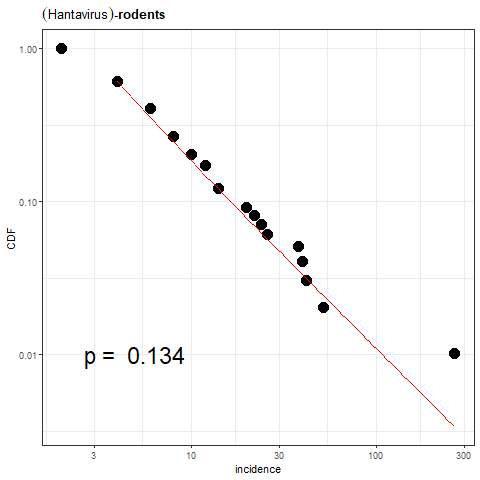
\includegraphics[width=0.5\textwidth]{01_fig_powerlaw}
    \caption{Hantavirus - rodents system model under this protocol}
    \label{fig:powerlaw}
\end{figure}

\begin{figure}[tbhp]
    \centering
    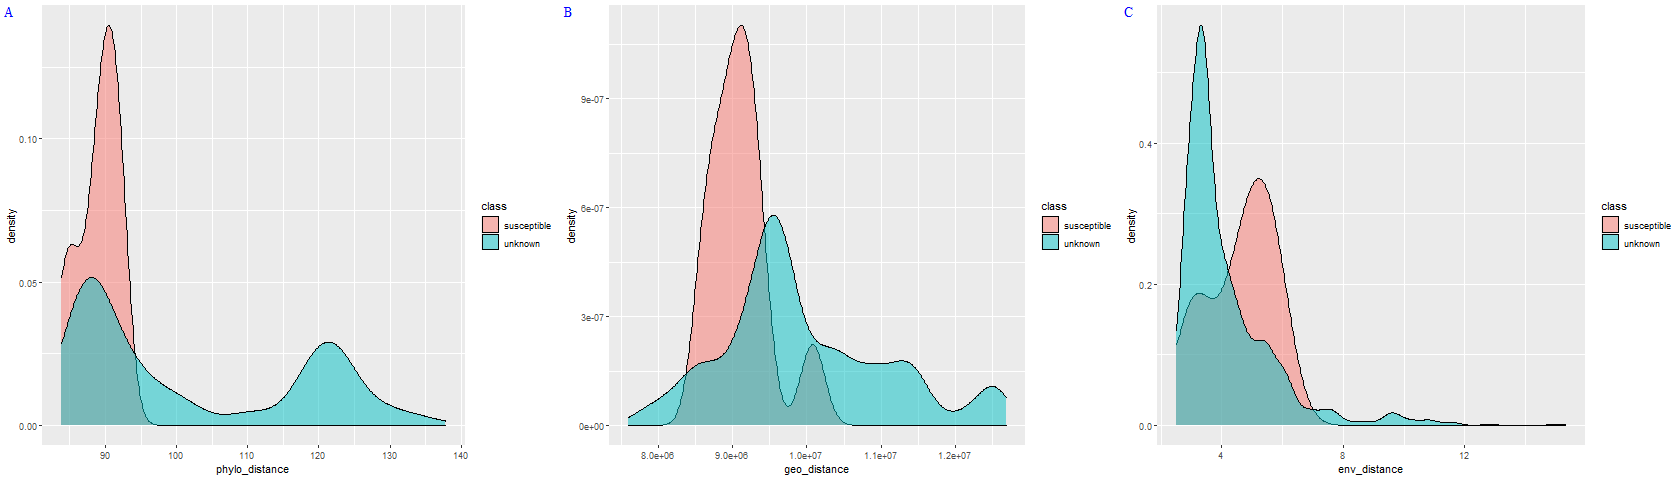
\includegraphics[width=1\textwidth]{02_density_functions.png}
    \caption{Density functions of distance for rodents that has been labeled as susceptible (i. e. one incidence recorded) and unknown (i. e. random sampled from the rodent species pool with no records)}
    \label{fig:density}
\end{figure}

\begin{figure}[tbhp]
    \centering
    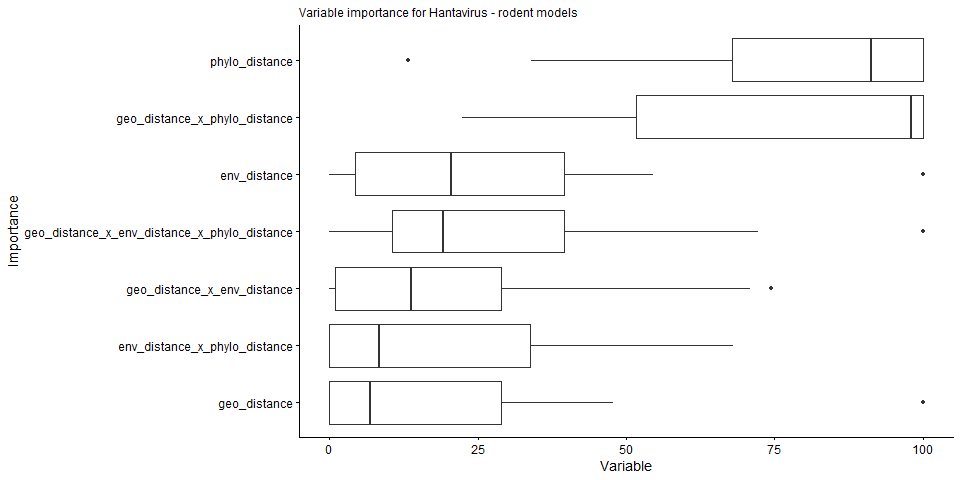
\includegraphics[width=0.75\textwidth]{03_vip_rodents.png}
    \caption{Variable importance from the models outputs after 1000 runs}
    \label{fig:vip}
\end{figure}

\begin{figure}[tbhp]
    \centering
    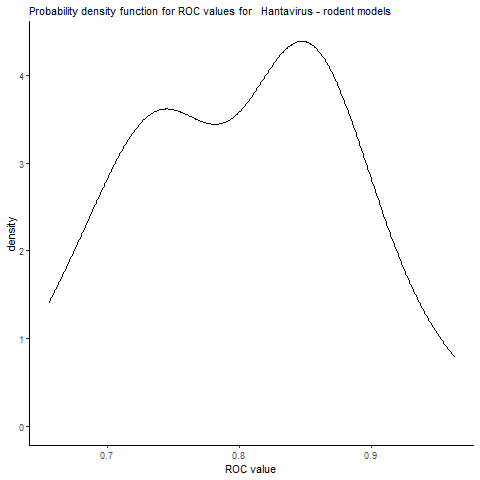
\includegraphics[width=0.75\textwidth]{04_p_roc_density.png}
    \caption{Probability density function of ROC values for each model}
    \label{fig:rocdensity}
\end{figure}
\begin{figure}[tbhp]
    \centering
    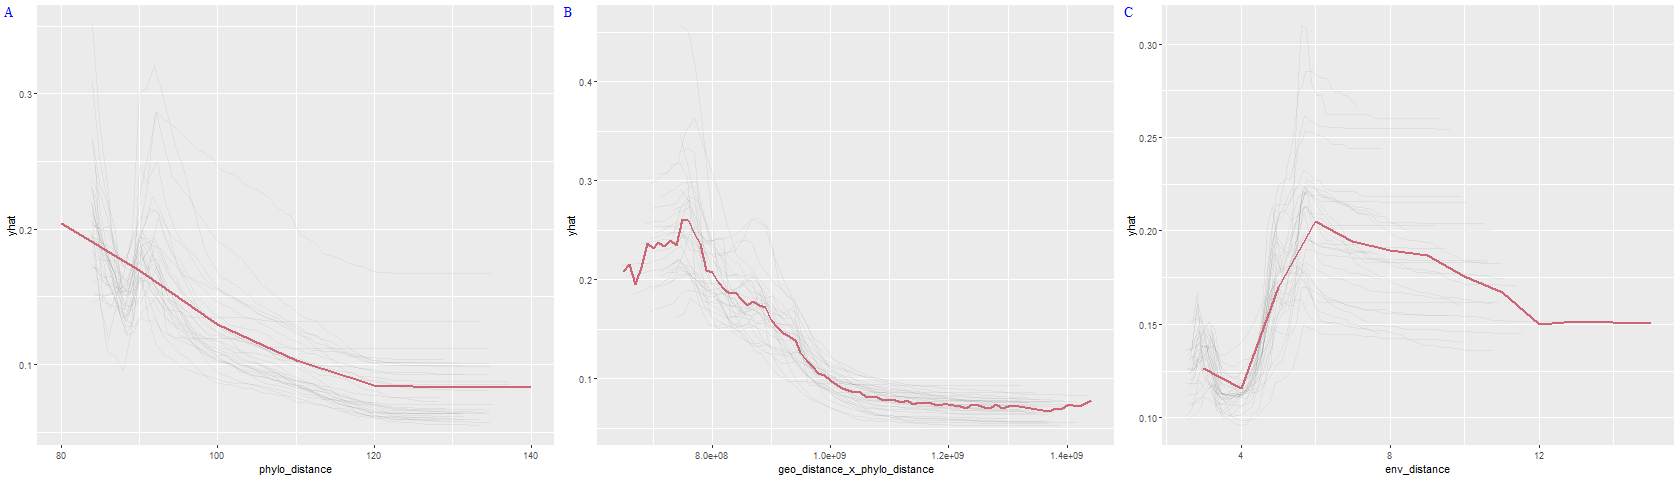
\includegraphics[width=1\textwidth]{05_pdp_top3.png}
    \caption{Partial dependent plots for the first most importan variables according to \ref{fig:vip}}
    \label{fig:density}
\end{figure}


\bibliographystyle{plain}
\bibliography{test}
\end{document}



\end{document}
